\documentclass[chapterprefix=false, 12pt, a4paper, oneside, parskip=half, listof=totoc, bibliography=totoc, numbers=noendperiod]{scrbook}

\usepackage[utf8]{inputenc}
\usepackage[T1]{fontenc}
\usepackage[bottom=48mm,left=25mm,right=25mm]{geometry}
\usepackage[onehalfspacing]{setspace}
\usepackage[stretch=10]{microtype}
\usepackage{xcolor}
\usepackage{scrhack}
\usepackage{titling}
\usepackage[outputdir=out]{minted}
\usepackage{graphicx}
\usepackage{hyperref}
\usepackage[ngerman]{babel}
\usepackage{biblatex}


\renewcommand*{\chapterheadstartvskip}{\vspace*{.25\baselineskip}}
\def\changemargin#1#2{\list{}{\rightmargin#2\leftmargin#1}\item[]}
\let\endchangemargin=\endlist

\definecolor{htwgruen}{RGB}{118, 185, 0}
\definecolor{htwblau}{RGB}{0, 130, 209}
\definecolor{htworange}{RGB}{255, 95, 0}
\definecolor{htwgrau}{RGB}{175, 175, 175}

\title{Bericht über Werkstudententätigkeit bei der DERICON GmbH}
\author{Christoph Stach}
\date{01.11.2016 bis 30.09.2018}

\addbibresource{main.bib}
\defbibheading{none}[\bibname]{
%%
}

\begin{document}
    \begin{titlepage}
        % Logo
        
\includegraphics[width=0.50\textwidth]{img/Q01_HTW_Berlin_Logo_quer_pos_FARBIG_CMYK.eps}

        % Abstand nach logo
        \vspace{4.0cm}

        % Textkörper
        \begin{changemargin}{0.5cm}{0.0cm}
            % Dokumenttyp
            \color{htwgrau}
            \normalsize
            \textsf{\noindent\MakeUppercase{Dokumenttyp}} \vspace{-20pt}\\
            % Horizontale Linie
            \noindent\rule{\textwidth}{0.5pt}\vspace{-4pt}
            % Title
            \color{black}
            \huge
            \textsf{Bericht über Werkstudententätig}
            \vspace{12pt}

            % Author
            \color{htwgrau}
            \normalsize
            \textsf{\MakeUppercase{Autor}}\\
            \color{black}
            \large
            \textsf{\theauthor}

            % Zeitraum
            \color{htwgrau}
            \normalsize
            \textsf{\MakeUppercase{Zeitraum}}\\
            \color{black}
            \large
            \textsf{\thedate}

            % Am Ende der Seite
            \vfill

            % Firma
            \color{htwgrau}
            \normalsize
            \textsf{\MakeUppercase{Firma}}\\
            \color{black}
            \large
            \textsf{DERICON GmbH}

            % Dozent
            \color{htwgrau}
            \normalsize
            \textsf{\MakeUppercase{Dozent}}\\
            \color{black}
            \large
            \textsf{Prof. Dr. Schüler}
            \vspace{-60pt}
        \end{changemargin}
    \end{titlepage}

    \tableofcontents

    \chapter{Allgemeines}

    Dieser Bericht behandelt die Werkstudententätigkeit von Christoph Stach bei der DERICON GmbH im Zeitraum vom 01.10.2016 bis 31.09.2018.

    \section{Beschreibung des Unternehmens}

    Die DERICON GmbH ist ein bankenunabhängiges Finanzdienstleistungsinstitut mit Standorten in Frankfurt am Main und Berlin.
    Das Unternehmen unterstützt seit 2008 Banken und Vermögensverwalter bei der Gestaltung effizienter und rechtskonformer Beratungs- und Vertriebsprozesse.
    Mit DERIFIN betreibt DERICON dafür die führende Webanwendung zur Selektion, Steuerung und Risikomanagement von strukturierten Produkten.
    Zudem liefert DERICON professionelle Daten und Kennzahlen für die Analyse und den Einsatz strukturierter Produkte.
    Europaweit vertrauen bereits mehr als 60 Privatbanken, Sparkassen und Genossenschaftsinstitute auf die Expertise von DERICON.
    \\ \\
    Im Jahr 2015 wurde über DERIFIN ein Anlagevolumen von rund 1,2 Mrd. Euro vermittelt.

    \section{Beschreibung der Produkte}

    Das Hauptprodukt von DERICON ist die Webanwendung DERIFIN. Außerdem wurde während ich bei der DERICON GmbH eingestellt war,
    eine neue Version von DERIFIN entwickelt, das sogenannte DERIFIN WMS, welches mehr Features bietet und mit neueren Technologien entwickelt wurde.
    Neben der Hauptsoftware DERIFIN entwickelt DERICON viele interne Produkte zur besseren Verwaltung von DERIFIN und seiner Kunden.

    \section{Beschreibung des Teams}

    Das Team von DERICON ist auf zwei Standorte verteilt. Der erste Standort ist in Frankfurt am Main und der zweite Standort in Berlin Charlottenburg.
    Mein Arbeitsplatz ist im Berliner Büro. Zum heutigen Zeitpunkt arbeiten zwei Frontend-Entwickler, sowie einer der Geschäftsführer in diesem Büro.
    Im Frankfurter Büro arbeiten überwiegend Backend-Entwickler sowie ein weiterer Geschäftsführer und die Buchhaltung.
    \\ \\
    Die komplette Entwicklungsabteilung hält jeden Morgen ein Meeting per Videotelefonie, in dem jedes Mitglied kurz berichtet
    was es am Vortag gemacht hat und was es an diesem Tag vorhat.
    Die Entwicklung ist in Sprints von zwei Wochen gegliedert. Deswegen gibt es ein weiteres Sprintplanungsmeeting am Anfang eines jeden Sprints.
    Dieser Prozess ist an SCRUM\footnote{Eine Methode für agiles Projektmanagement.} angelehnt.

    \section{Organisation}

    \subsection{Issue-Management}

    Die Aufgabenverteilung ist über die Software JIRA\footnote{Eine Webanwendung für das Projektmanagement und die Fehlerverwaltung von Software. \\ Link: \url{https://www.atlassian.com/software/jira}} geregelt.
    Alle neuen Features sowie anfallende Fehler werden hier gespeichert.
    Bei der Sprintplanung wird besprochen, welche Issues\footnote{In JIRA werden Fehler, Features und andere Artefakte generell als Issues bezeichnet.}
    im kommenden Sprint umgesetzt werden sollen. Die Issues werden über den Sprint vom Teamleader an die einzelnen Entwickler verteilt. Auch ist es möglich sich, selbst Issues zuzuweisen.

    \pagebreak

    \subsection{Versionskontrolle}

    Alle Software Projekte werden in GIT-Repositories\footnote{Eine Versionskontrollsystem entwickelt von Linus Torvalds. Link: \url{https://git-scm.com}} \\
    auf \url{https://bitbucket.org} verwaltet.
    Wird ein Issue aus JIRA von einem Entwickler fertiggestellt, wird auf BitBucket ein Pull-Request auf den Development-Branch erstellt.
    Dieser muss erst von anderen Entwicklern überprüft werden, bevor er endgültig in den Development-Branch der Software
    gemerged wird.

    \subsection{Buildmanagement}

    Alle Applikationen werde über JENKINS\footnote{Ein Server zur Automatisierung von Aufgaben, wird oft für den Buildprozess von Software eingesetzt. Link: \url{https://jenkins.io}} gebaut.
    Treten keine Fehler beim Buildprozess auf, werden diese danach von JENKINS auf die Server bei Amazon AWS\footnote{Hostingservice für Server und andere Services der Firma Amazon. Link: \url{https://aws.amazon.com}} kopiert.

    \chapter{Aufgaben}

    Während meiner Zeit bei der DERICON GmbH habe ich überwiegend an drei verschiedenen Softwareprodukten gearbeitet.
    Meine Arbeit bezog sich meistens auf die Implementierung neuer Features und das Beheben von Fehlern. In den Unterpunkten \textbf{Entwicklung}
    werde ich jeweils auf einige JIRA-Issues mit einer kurzen Beschreibung referenzieren.

    \section{CitrusNG}

    \subsection{Ausgangsposition}

    CitrusNG war das erste Projekt an dem ich mitgewirkt habe. Es ist ein internes Produkt für die Konfiguration der unterschiedlichen DERIFIN Umgebungen, die
    vom Kunden benutzt werden. Jeder Kunde hat unterschiedliche Wünsche. Deswegen ist die DERIFIN Software sehr stark konfigurierbar.
    Um die Konfigurationen einfacher zu verwalten gibt es CitrusNG.

    CitrusNG ist eine Webanwendung. Das Frontend ist mit AngularJS (Version 1)\footnote{JavaScript Framework für die Erstellung von
    Single Page Apps. Link: \url{https://angularjs.org}} implementiert.
    Das Backend mit SpringBoot\footnote{Java Framework der Firma Pivotal. Link: \url{http://spring.io/projects/spring-boot}} Micro-Services.
    Zwischen Backend und Frontend wird eine weitere PHP-Ebene mit Symfony\footnote{Symfony ist ein weitverbreitetes
    PHP Framework mit wiederverwendtbaren Bibliotheken und Komponenten der Firma SensioLabs. Link: \url{https://symfony.com}}
    implementiert, welche in Form einer Middleware eingesetzt wird. Die Middleware und das Frontend werden von den Frontent-Entwicklern gepflegt.
    Das Ziel der Middleware ist es den Frontend-Entwicklern die Möglichkeit zu geben, die Ergebnisse der
    Backend-Endpunkte zu manipulieren und sie angepasst an das Frontend weiterzuleiten. 
    Hier werden beispielsweise unnötige JSON\footnote{JavaScript Object Notation: Ein Format für die Übertragung von
    Objekten zwischen Server und Client Anwendungen}-Felder entfernt oder
    aggregiert, Mock-Daten generiert oder Sortierfunktionen implementiert.

    \begin{center}
        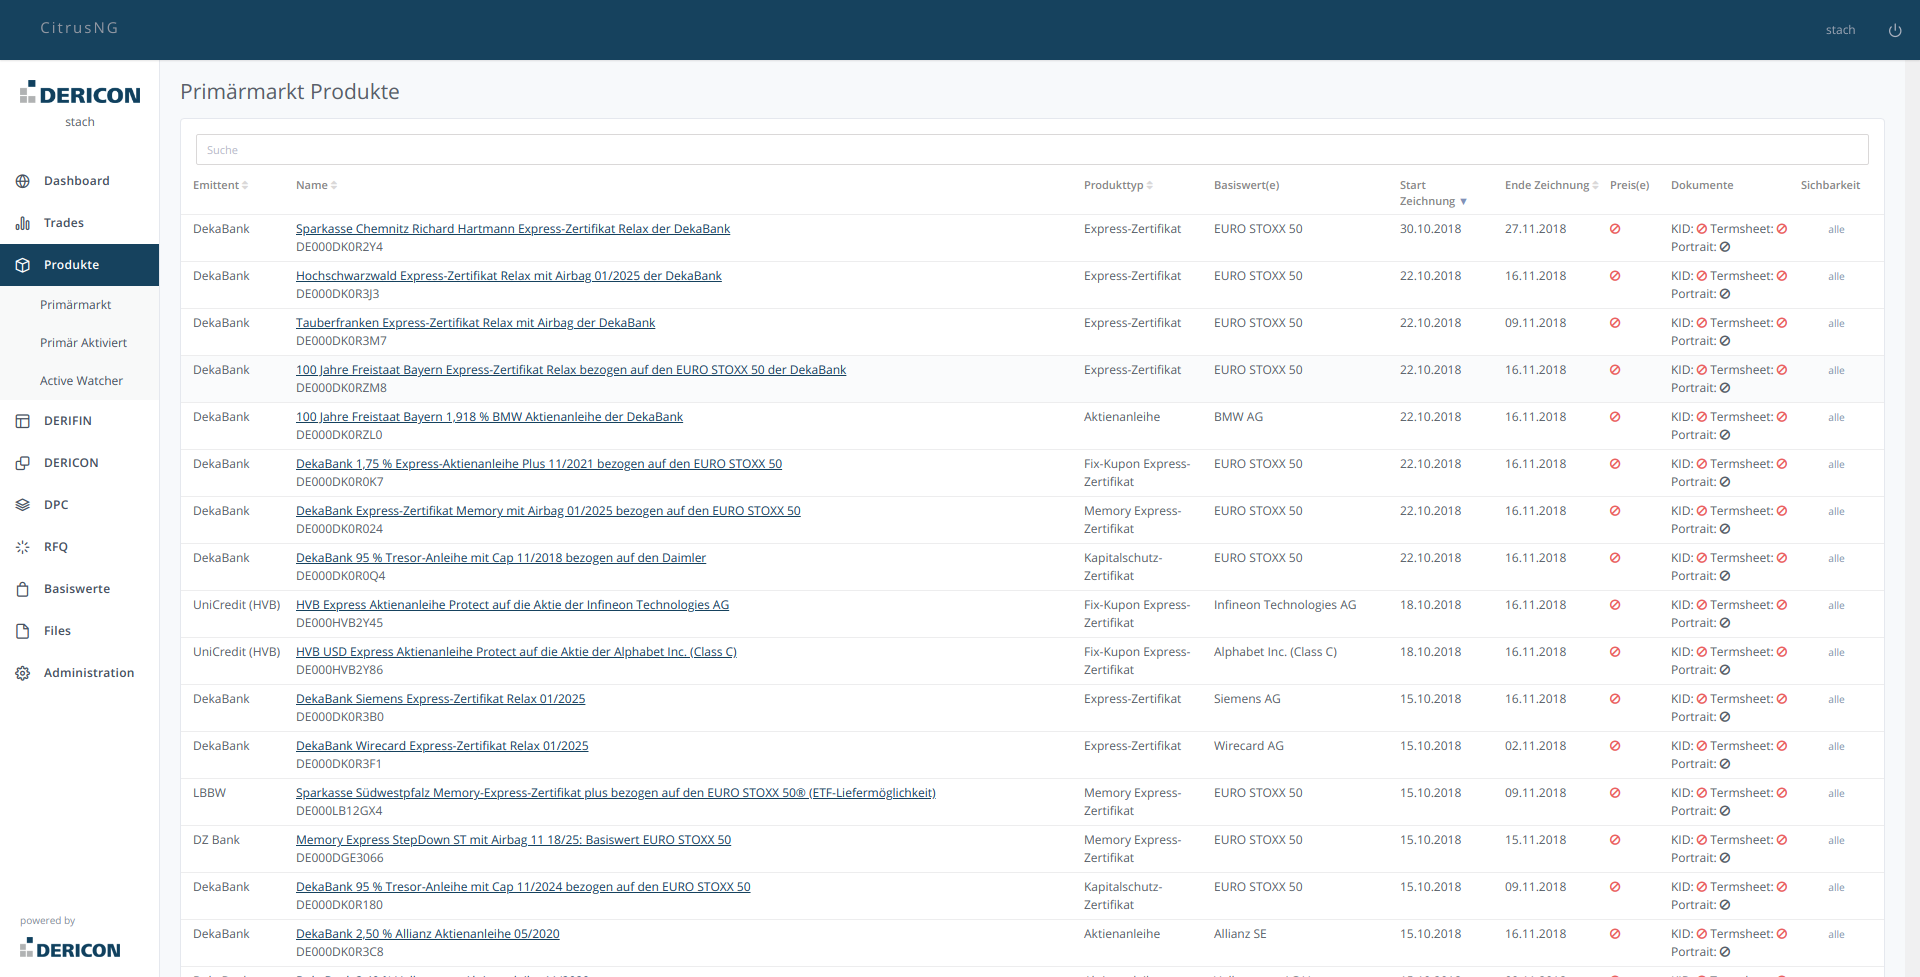
\includegraphics[width=0.75\textwidth]{img/citrusng.png}
        \captionof{figure}{Screenshot der Software CitrusNG}
    \end{center}

    \subsection{Entwicklung}

    An CitrusNG habe ich unterschiedliche Aufgaben verrichtet. Ich habe insgesamt ca. 1 Jahr an diesem Projekt mitgewirkt.
    Im Folgenden zähle ich einige Beispiele meiner Arbeit auf.

    \subsubsection{CNG-319: Möchten Sie wirklich die Seite verlassen? Sie haben noch ungespeicherte Änderungen!}

    Es sollte bei diesem Feature eine Bestätigung implementiert werden, welche angezeigt wird, wenn bereits Änderungen an einem Formular
    gemacht worden sind und diese vom Benutzer nicht gespeichert wurden, bevor er die Seite verlässt.

    Sobald Änderungen am Formular vorliegen, muss eine Variable \textit{vm.saved} auf \textit{false} gesetzt werden.

    \begin{minted}[xleftmargin=20pt,linenos,breaklines]{javascript}
    function changed() {
        vm.saved = false;
    }
    \end{minted}

    Außerdem muss die Variable \textit{\$scope} überwacht werden. Darüber kann bei AngularJS überprüft werden, ob der
    Benutzer die aktuelle Seite verlassen will, und man kann auf dieses Ereignis reagieren.

    \begin{minted}[xleftmargin=20pt,linenos,breaklines]{javascript}
    function DividendsController(apiClient, \$q, \$state, \$scope) {
        var vm = this;
        vm.saved = false;

        function onStateChange(event, toState, toParams) {
            if (!vm.saved) {
                if (!confirm('Wollen Sie die Seite...?')) {
                    event.preventDefault();
                }
            }
        }
    }
    \end{minted}

    \subsubsection{CNG-381: DPC Emittierte Produkte - Liste sortierbar machen}

    In diesem Issue sollte, wie der Titel sagt, eine Tabelle von Finanzprodukten sortierbar gemacht werden.
    Die zu dem Zeitpunkt bereits bestehende Tabelle benutzt das AngularJS-Plugin Smart Table\footnote{Link: \url{http://lorenzofox3.github.io/smart-table-website/}}.
    Das Plugin bietet die Möglichkeit, einfach dynamisch generierte Tabellen zu erstellen. Es bietet außerdem eine Angular Directive, um die Tabellen-Spalten sortierbar zu machen.

    \begin{minted}[xleftmargin=20pt,linenos,breaklines]{html}
    <th>
        <div st-sort="environmentData.name" class="th-label">
            Umgebung Name <i class="fa fa-sort"></i>
        </div>
    </th>
    \end{minted}

    Zur Umsetzung der Aufgabe habe ich lediglich die entsprechende \textit{st-sort} Directive zu den zu sortierenden
    Spalten sowie ein Sortier-Icon hinzugefügt.

    \pagebreak

    Der Wert der Directive entspricht dem Key im JavaScript-Objekt nach dem
    sortiert werden soll.

    \subsection{Ergebnisse}

    Während meiner Arbeit an CitrusNG habe ich insgesamt 40 JIRA-Issues bearbeitet. Dabei handelte
    es sich um das Beheben von Fehlern in der Software sowie auch der Implementierung neuer Features.

    \section{BrokerUI}

    \subsection{Ausgangsposition}

    Die DERICON GmbH hatte sich entschieden, ihr Hauptprodukt \textbf{DERIFIN} neu zu entwickeln.
    Das Projekt wurde jedoch nicht intern entwickelt, sondern von einem externen Softwareentwicklungs Dienstleister.
    Das neue \textbf{DERIFIN WMS} sollte als hoch konfigurierbares System entwickelt werden, um den vielfältigen
    Kundenwünschen der DERICON GmbH zu entsprechen. Das Ziel war, es jegliche Konfiguration der Software in einem
    Datanbanksystem zu hinterlegen, um diese für jeden Kunden dynamisch anpassbar zu machen.

    \begin{center}
        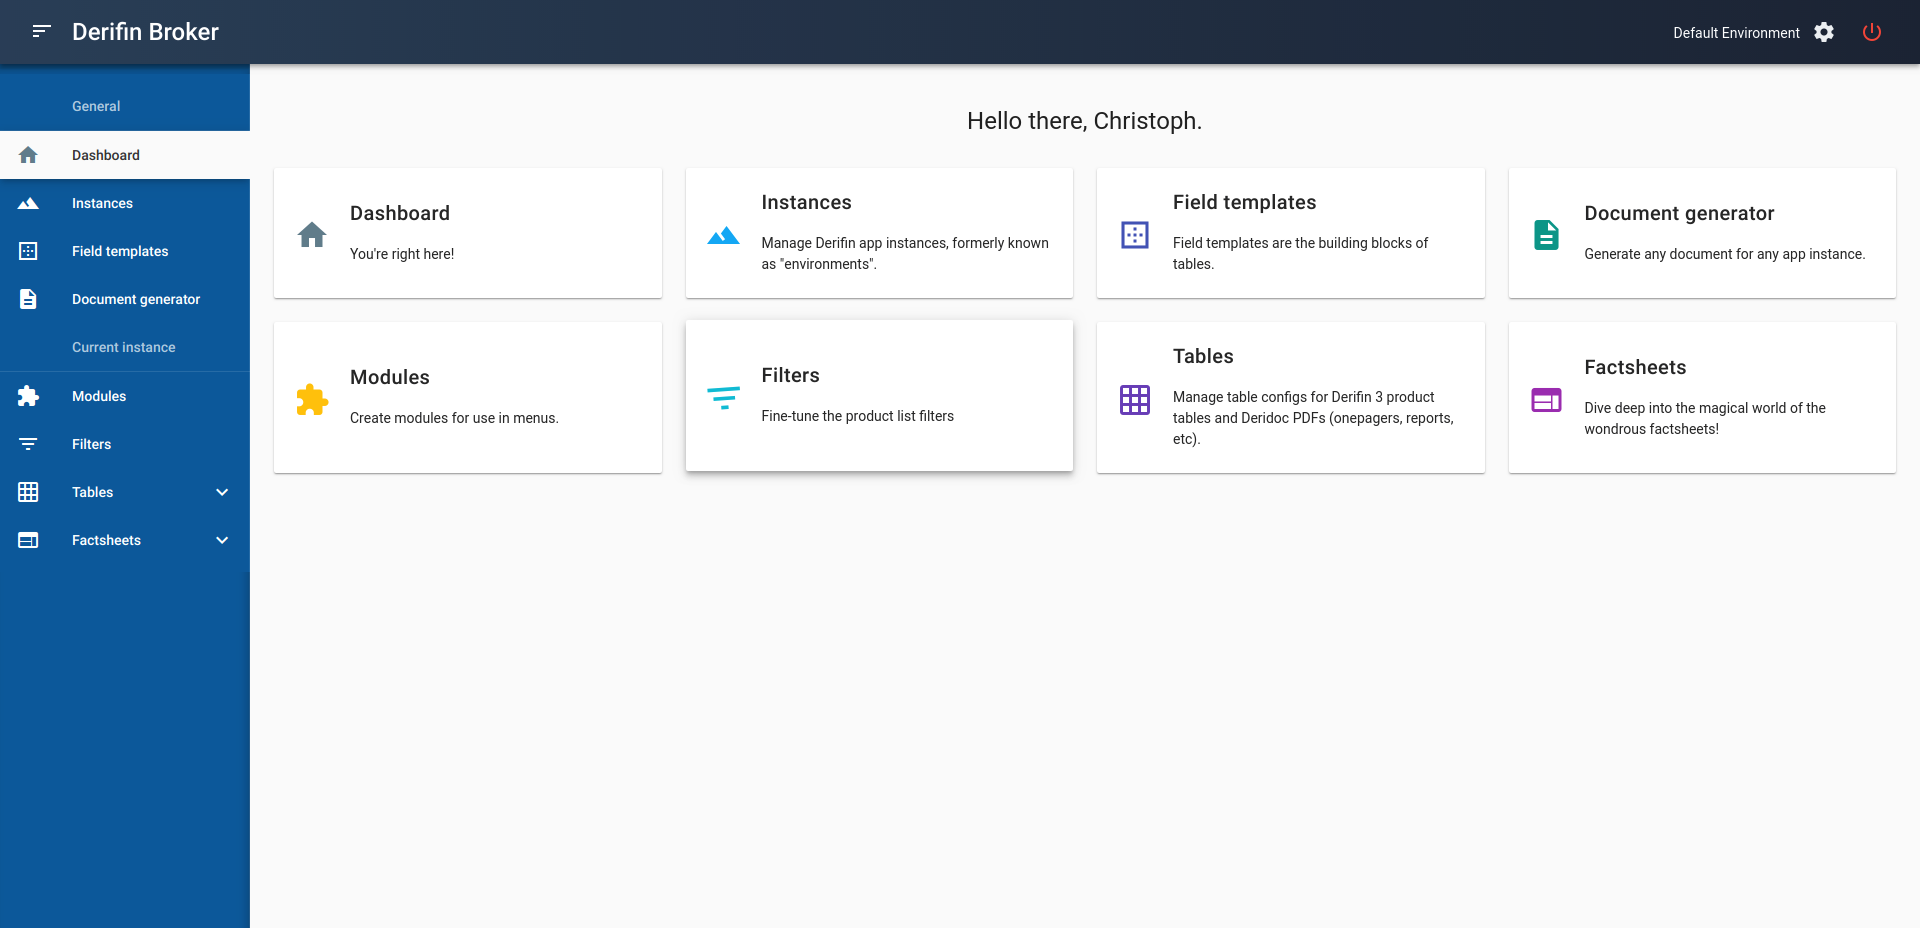
\includegraphics[width=0.75\textwidth]{img/broker-ui-neu.png}
        \captionof{figure}{Screenshot der Software BrokerUI}
    \end{center}

    Damit die Mitarbeiter der DERICON GmbH diese Konfigurationen für Ihre Kunden leicht verwalten können, sollte eine
    weitere Software von Grund auf neu entwickelt werden. Diese Software wurde BrokerUI genannt und ich wurde mit der
    Entwicklung beauftragt.

    \subsection{Entwicklung}

    Auf dem oben gezeigten Screenshot sieht man den BrokerUI zum Zeitpunkt der Erstellung der Dokumentation. Dabei wurden folgende
    Punkte größtenteils von mir entwickelt. Da die DERICON GmbH auf ihrer Derifin WMS Plattform unterschiedliche Finanzmarktprodukte
    wie Aktion, Anleihen usw. vertreibt, dienen diese Punkte der Konfiguration der unterchiedlichen Ansichten der Finanzprodukte im
    Frontend.

    \subsubsection{Menus}

    Jeder Kunde kann eine eigene auf sich zugeschnittene Menüstruktur haben.
    Dabei werden Menüpunkte mit Modulen verknüpft.

    \subsubsection{Modules}

    Im Punkt Modules können unterschiedliche Modulkonfigurationen erstellt werden. Diese Modulkonfiguration sind das \textit{Herzstück}
    von DERIFIN WMS, da Sie bestimmen wie die unterschiedlichen Ansichten im Frontend beim Kunden angezeigt werden.

    \subsubsection{Translations}

    Hier können unterschiedliche String-Label die im Frontend benutzt werden konfiguriert werden, damit wir jedem Kunde
    die Software mit seinen gewünschten Texten versehen können.

    \subsubsection{Tables}

    Tables sind spezielle Module die Tabellen von unterschiedlichen Finanzprodukten anzeigen können.

    \subsubsection{Factsheets}

    Ein Factsheet (auch Produkteinzelansicht genannt) ist eine Übersichtseite über ein Finanzprodukt. Diese kann auch je nach Kunde unterschiedlich zusammengestellt sein.
    Hier können Diagramme und Warnmeldung für das Finanzprodukt konfiguriert werden. Siehe Abbildung 2.3.

    \subsection{Ergebnisse}

    Wie im Vorfeld erwähnt, wurden die oben aufgezählten Features von mir implementiert. Im weiteren Verlauf habe ich das Projekt
    abgegeben. Es wurden noch weitere Features implementiert, das Design geändert und vom Angular Framework
    auf das Vue.js\footnote{Vue.js ist ähnlich wie Angular ein JavaScript Frontend Framework. Link: \url{https://vuejs.org}}
    Framework umgestellt.

    \section{DERIFIN WMS}

    \subsection{Ausgangsposition}

    Nach meiner Arbeit am \textbf{BrokerUI} war es meine Aufgabe, mich in das vom externen Softwaredienstleister
    entwickelte DERIFN WMS einzuarbeiten. Das Projekt war zu großen Teilen fertiggestellt und sollte, bevor es an die
    Kunden ausgeliefert wurde, noch einen Feinschliff erhalten. Fehlende Features sollten implementiert werden und bestehende
    Fehler behoben werden. Außerdem sollte das Projekt von Angular Version 4 auf Angular Version 6 aktualisiert werden, damit
    es weiterhin zukunftsfähig und erweiterbar bleibt.

    \begin{center}
        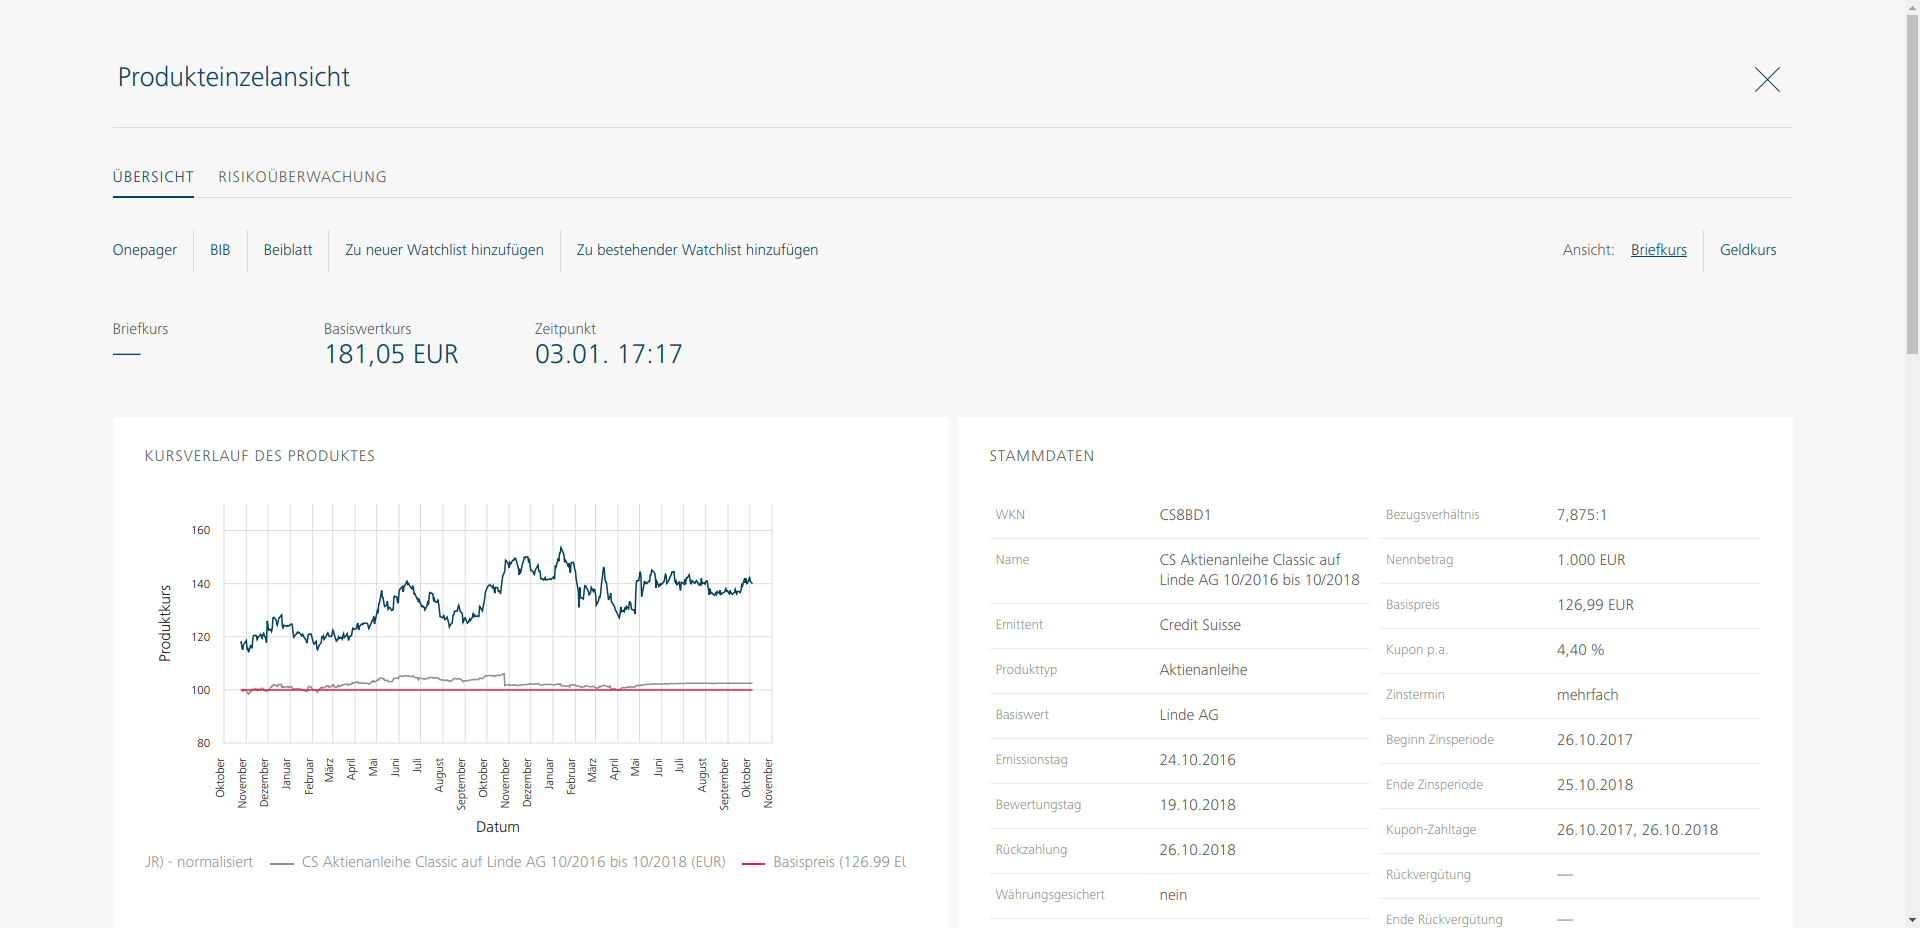
\includegraphics[width=0.75\textwidth]{img/derifin.png}
        \captionof{figure}{Screenshot der Software DERIFIN WMS}
    \end{center}

    Aufgrund seiner hohen Konfigurierbarkeit, ist das DERIFIN WMS sehr dynamisch aufgebaut. Der Großteil der HTML Komponenten
    wird dynamisch im Frontend generiert und ist durch die im Backend gespeicherten Daten konfigurierbar. Ich wurde mit
    der Weiterentwicklung beauftragt, weil ich zu dem Zeitpunkt bereits die meisten Erfahrungen mit dem Angular Framework gesammelt hatte.

    \subsection{Entwicklung}

    \subsubsection{DFN-547: Download eines Historischen Universums}

    Aufgrund einer Gesetzesänderung müssen Banken nachweisen, welche Produkte Sie ihren Kunden in der Vergangenheit
    angeboten haben. Deswegen musste eine Historienfunktion implementiert werden.

    Im Folgenden habe ich ein Formular erstellt, welches die Eingabe eines Daten-Zeitraums erlaubt. Dieser Zeitraum wird zum
    Backend geschickt, welches mit einer Liste von Finanzprodukten antwortet, die in diesem Zeitraum als Auswahl zur Verfügung
    stand. Zusätzlich kann über das Aufrufen eines anderen Endpunktes eine Excel-Liste generiert werden. Das Backend generiert
    diese Liste und antwortet dem Frontend mit einer URL zur Liste, welche dann durch das Frontend aufgerufen wird, um den
    Download der Excel-Datei zu starten.

    \subsubsection{DFN-486: Ladebalken für Produkteinzelansicht}

    Die Produkteinzelansicht (in Abbildung 2.3 zu sehen) wird je nach Kundenkonfiguration dynamisch generiert.
    Die Daten über das Aussehen der Ansicht werden vom Backend über den sogenannten \textit{structure}-Endpunkt geliefert.
    Der \textit{data}-Endpunkt liefert die eigentlichen Daten, die in den HTML Komponenten, die gemäß des \textit{structure}-Endpunktes
    generiert werden, angezeigt werden müssen. Alle vom Backend empfangenen Daten werden im Frontend gemäß des
    REDUX\footnote{Store-Pattern auf einem \textit{Single source of truth}-Prinzip basiert. Link: \url{https://redux.js.org}}-Pattern gespeichert.
    Dieses ist in Angular über die Bibliothek \textit{ngrx}\footnote{Link: \url{https://github.com/ngrx}} implementiert.
    Alle Daten die im \textit{ngrx}-Store gespeichert sind, können in den Komponenten auf Änderungen überwacht werden.

    Ich habe dem Store zwei neue Eigenschaften hinzugefügt, welche den Ladestatus der beiden Endpunkte wiederspiegeln.
    Dadurch war es mir möglich, die beiden \textit{Observables} der Eigenschaften in der Produkteinzelansicht zu überwachen.
    Nur in dem Fall, in dem der Ladestatus beider auf \textit{false} steht, wird der Inhalt der Produkteinzelansicht angezeigt.
    Sonst wird ein Ladebalken gezeigt. Das hat zur Folge das beim Laden der Produkteinzahlansicht dem Benutzer zuerst ein Ladebalken
    angezeigt wird, solange bis alle notwendingen Daten zum korrekten Anzeigen der Ansicht vorhanden sind.


    \subsection{Ergebnisse}

    Nach der Behebung einiger Fehler, Aktualisierung auf Angular Version 6 und der Entwicklung mehrerer Features,
    wurde das neue DERIFIN WMS bereits an drei unserer Kunden ausgeliefert. Die bisherigen Rückmeldungen der Kunden sind positiv.

    \chapter{Schlussfolgerungen}

    \section{Zusammenhänge mit dem Studium an der HTW Berlin}

    Durch meine Arbeit bei der DERICON GmbH konnte ich mein Wissen besonders im Bereich der Webentwicklung erweitern.
    Ich konnte viele Ansätze, die im Modul \textit{Webentwicklung} an der HTW  Berlin geleehrt werden, anwenden. Ich habe die zwei Frameworks
    AngularJS und Angular kennengelernt. Besonders durch die Arbeit mit Angular konnte ich Parallelen zum Studium ziehen. Angular
    verwendet verstärkt die Bibliothek \textit{rxjs}, welche das Observable-Pattern implementiert. Dieses wurde bereits im Modul
    \textit{Programmierung 3} an der HTW Berlin behandelt. Außerdem arbeitet man viel mit Functional Programming Methoden, die auch bereits in Form
    von Streams in \textit{Programmierung 3} sowie im Modul \textit{Entwicklung sozialer Anwendungen} gelehrt wurden.

    Bei meiner Arbeit an der Software \textit{CitrusNG} habe ich viel mit dem MVC-Paradigma gearbeitet. Dieses wird bei \textit{Symfony}
    und \textit{AngularJS} viel verwendet. Dadurch konnte ich Verbindungen zu den Modulen \textit{Webentwicklung} und \textit{Programmierung 3}
    sowie \textit{Software Engineering} herstellen.

    % \chapter{Anhang}

    % \section{Literaturverzeichnis}

    % \printbibliography[heading=none]

    % \section{Glossar}
\end{document}
